% TODO checklist:
% - [x] README.md: Database descriptions, persistence patterns
% - [x] Q&A.md (Section B, Q10-Q12): Repository pattern, Redis usage, Memgraph role
% - [x] Q&A.md (Section E, Q29-Q35): Graph data model, NL-to-Cypher
% - [x] db/postgres_control/: PostgreSQL models and repositories
% - [x] db/redis/: Redis client and caching patterns
% - [x] db/memgraph_domain/: Graph schema and queries

\section{Data and Persistence Layer}
\label{sec:data-layer}

The Data and Persistence Layer implements a polyglot persistence strategy, employing three specialized databases to address distinct requirements: PostgreSQL for authoritative state and transactional integrity, Redis for high-performance caching and real-time operations, and Memgraph for graph-based knowledge representation and querying. This section details the design and implementation of each data store.

\subsection{PostgreSQL Control Plane}
\label{subsec:postgresql}

PostgreSQL serves as the \textbf{control plane} database, storing all authoritative state including tenants, users, agent runs, jobs, model configurations, and audit logs. The platform uses SQLAlchemy 2.0 as the ORM with Alembic for schema migrations.

\paragraph{Database Schema Overview}
The PostgreSQL schema comprises 15+ tables organized by domain. Figure~\ref{fig:postgres-schema} illustrates the core entity relationships.

\begin{figure}[htbp]
    \centering
    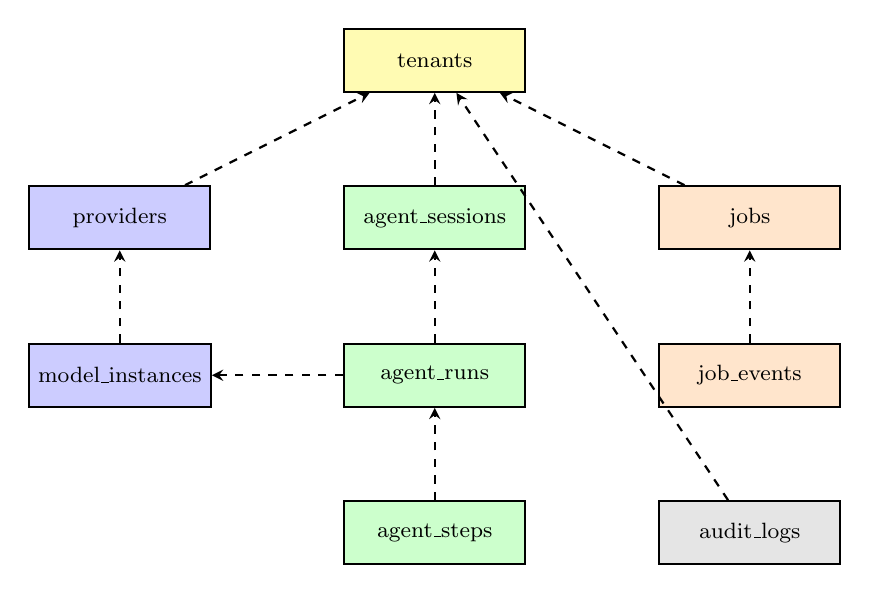
\begin{tikzpicture}[
        node distance=1.5cm,
        table/.style={rectangle, draw=black, thick, minimum width=2.3cm, minimum height=0.8cm, align=center, font=\footnotesize},
        pk/.style={font=\tiny\bfseries},
        fk/.style={->, thick, >=stealth, dashed}
    ]
        % Core tables
        \node[table, fill=yellow!30] (tenant) at (0, 4) {tenants};
        \node[table, fill=blue!20] (provider) at (-4, 2) {providers};
        \node[table, fill=blue!20] (model) at (-4, 0) {model\_instances};
        \node[table, fill=green!20] (session) at (0, 2) {agent\_sessions};
        \node[table, fill=green!20] (run) at (0, 0) {agent\_runs};
        \node[table, fill=green!20] (step) at (0, -2) {agent\_steps};
        \node[table, fill=orange!20] (job) at (4, 2) {jobs};
        \node[table, fill=orange!20] (event) at (4, 0) {job\_events};
        \node[table, fill=gray!20] (audit) at (4, -2) {audit\_logs};
        
        % Relationships
        \draw[fk] (provider) -- (tenant);
        \draw[fk] (model) -- (provider);
        \draw[fk] (session) -- (tenant);
        \draw[fk] (run) -- (session);
        \draw[fk] (run) -- (model);
        \draw[fk] (step) -- (run);
        \draw[fk] (job) -- (tenant);
        \draw[fk] (event) -- (job);
        \draw[fk] (audit) -- (tenant);
    \end{tikzpicture}
    \caption{Core PostgreSQL schema showing table relationships.}
    \label{fig:postgres-schema}
\end{figure}

\paragraph{Table Inventory}
Table~\ref{tab:postgres-tables} provides a complete inventory of PostgreSQL tables with their purposes and key columns.

\begin{table}[htbp]
    \centering
    \caption{PostgreSQL table inventory.}
    \label{tab:postgres-tables}
    \small
    \begin{tabularx}{\textwidth}{llX}
        \toprule
        \textbf{Table} & \textbf{Key Columns} & \textbf{Purpose} \\
        \midrule
        \texttt{tenants} & id, name, slug, config\_json & Organizational units \\
        \texttt{providers} & id, name, api\_type, base\_url & LLM provider configs \\
        \texttt{model\_instances} & id, instance\_name, model\_name & Model deployments \\
        \texttt{agent\_sessions} & id, owner\_sub, context\_json & Conversation containers \\
        \texttt{agent\_runs} & id, status, prompt, final\_answer & Orchestration executions \\
        \texttt{agent\_steps} & id, run\_id, action, tool\_name & Execution steps \\
        \texttt{jobs} & id, type, status, payload\_json & Background tasks \\
        \texttt{job\_events} & seq\_id, job\_id, event\_type & Job state changes \\
        \texttt{audit\_logs} & id, actor\_sub, action, resource & Security audit trail \\
        \texttt{rate\_limits} & id, scope, limit, window & Rate limit configs \\
        \texttt{tool\_invocations} & id, tool\_name, input\_json & Tool call records \\
        \texttt{user\_preferences} & id, user\_sub, preferences\_json & User settings \\
        \texttt{tenant\_defaults} & id, tenant\_id, defaults\_json & Tenant configurations \\
        \texttt{manifests} & id, version, manifest\_json & Built-in model manifests \\
        \texttt{alembic\_version} & version\_num & Migration state \\
        \bottomrule
    \end{tabularx}
\end{table}

\paragraph{Schema Design Principles}
\begin{itemize}
    \item \textbf{UUID Primary Keys}: All tables use UUID v4 for primary keys, avoiding sequence contention and enabling distributed ID generation.
    \item \textbf{Tenant Scoping}: All user-facing tables include \texttt{tenant\_id} foreign key with cascading deletes.
    \item \textbf{JSONB Flexibility}: Complex, evolving data (configurations, metadata, tool I/O) uses JSONB columns.
    \item \textbf{Timestamp Tracking}: All tables include \texttt{created\_at} and \texttt{updated\_at} with automatic updates.
    \item \textbf{Soft Deletes}: Critical tables support soft deletion via \texttt{deleted\_at} column.
\end{itemize}

\paragraph{Migration Strategy}
The platform uses Alembic for declarative schema migrations, with 26 migrations tracking the schema evolution:

\begin{lstlisting}[language=Python, caption={Example Alembic migration for adding job events table.}]
def upgrade():
    op.create_table(
        'job_events',
        sa.Column('seq_id', sa.BigInteger, primary_key=True, autoincrement=True),
        sa.Column('job_id', postgresql.UUID(as_uuid=True), 
                  sa.ForeignKey('jobs.id', ondelete='CASCADE'), nullable=False),
        sa.Column('event_type', sa.String(100), nullable=False),
        sa.Column('event_json', postgresql.JSONB, default=dict),
        sa.Column('created_at', sa.DateTime(timezone=True), 
                  server_default=sa.func.now()),
    )
    op.create_index('ix_job_events_job_id', 'job_events', ['job_id'])

def downgrade():
    op.drop_table('job_events')
\end{lstlisting}

\subsubsection{Repository Pattern Implementation}
\label{subsubsec:repository-pattern}

The platform implements the Repository pattern to abstract data access, providing a consistent interface for CRUD operations while enabling testability through mock implementations.

\paragraph{Repository Architecture}
Each domain entity has a dedicated repository class in \texttt{db/postgres\_control/repositories/}:

\begin{lstlisting}[language=Python, caption={Repository base class and implementation pattern.}]
from abc import ABC, abstractmethod
from typing import Generic, TypeVar
from sqlalchemy.orm import Session

T = TypeVar('T')

class BaseRepository(ABC, Generic[T]):
    """Abstract base for all repositories."""
    
    def __init__(self, db: Session, tenant_id: str | None = None):
        self.db = db
        self.tenant_id = tenant_id
    
    @abstractmethod
    def get(self, id: UUID) -> T | None:
        pass
    
    @abstractmethod
    def create(self, entity: T) -> T:
        pass
    
    @abstractmethod
    def update(self, entity: T) -> T:
        pass
    
    @abstractmethod
    def delete(self, id: UUID) -> bool:
        pass
\end{lstlisting}

\paragraph{Repository Inventory}
Table~\ref{tab:repository-inventory} lists the repository classes and their responsibilities.

\begin{table}[htbp]
    \centering
    \caption{Repository classes and responsibilities.}
    \label{tab:repository-inventory}
    \small
    \begin{tabular}{ll}
        \toprule
        \textbf{Repository} & \textbf{Responsibilities} \\
        \midrule
        \texttt{TenantRepository} & Tenant CRUD, configuration management \\
        \texttt{ProviderRepository} & Provider registration, health status \\
        \texttt{ModelInstanceRepository} & Model instance management, usage tracking \\
        \texttt{AgentRunRepository} & Run persistence, status transitions, step recording \\
        \texttt{SessionRepository} & Session lifecycle, context management \\
        \texttt{JobRepository} & Job CRUD, queue management, idempotency \\
        \texttt{AuditLogRepository} & Append-only audit records, compliance queries \\
        \texttt{ToolInvocationRepository} & Tool call logging, error tracking \\
        \texttt{RateLimitRepository} & Quota configuration, override management \\
        \texttt{UserPreferencesRepository} & User settings, default model preferences \\
        \bottomrule
    \end{tabular}
\end{table}

\paragraph{Tenant-Scoped Queries}
All repositories automatically scope queries to the current tenant:

\begin{lstlisting}[language=Python, caption={Tenant-scoped query implementation.}]
class AgentRunRepository(BaseRepository[AgentRun]):
    def list_runs(
        self,
        status: str | None = None,
        limit: int = 20,
        cursor: str | None = None,
    ) -> list[AgentRun]:
        query = self.db.query(AgentRun)
        
        # Automatic tenant scoping
        if self.tenant_id:
            query = query.filter(AgentRun.tenant_id == self.tenant_id)
        
        if status:
            query = query.filter(AgentRun.status == status)
        
        if cursor:
            cursor_data = decode_cursor(cursor)
            query = query.filter(AgentRun.created_at < cursor_data['created_at'])
        
        return query.order_by(AgentRun.created_at.desc()).limit(limit).all()
\end{lstlisting}

\paragraph{Transaction Management}
Repositories participate in SQLAlchemy session transactions:

\begin{lstlisting}[language=Python, caption={Transaction management in service layer.}]
from contextlib import contextmanager

@contextmanager
def transaction(db: Session):
    try:
        yield db
        db.commit()
    except Exception:
        db.rollback()
        raise

# Usage in service
with transaction(db) as session:
    run = run_repo.create(new_run)
    for step in steps:
        step_repo.create(step)
    audit_repo.log_action("run.create", run.id)
\end{lstlisting}

\subsection{Redis Data Plane}
\label{subsec:redis}

Redis serves as the \textbf{data plane} database, providing high-performance caching, job queuing, rate limiting, and real-time state management. The platform uses Redis 7.x with the \texttt{redis-py} async client.

\paragraph{Design Rationale}
Redis complements PostgreSQL by handling:
\begin{itemize}
    \item \textbf{Hot data}: Frequently accessed data with sub-millisecond requirements
    \item \textbf{Ephemeral state}: Session tokens, rate limit windows, circuit breaker state
    \item \textbf{Pub/Sub}: Real-time event distribution (job updates, SSE)
    \item \textbf{Queues}: Job queuing with priority support
\end{itemize}

\subsubsection{Redis Usage Categories}
\label{subsubsec:redis-usage}

The platform employs Redis across ten distinct usage categories, each with specific key patterns and data structures.

\paragraph{1. Job Queues}
Jobs are queued using Redis lists with priority-based selection:

\begin{lstlisting}[language=Python, caption={Redis job queue implementation.}]
# Key pattern: jobs:queue:{job_type}
# Data structure: List (LPUSH/BRPOP)

async def queue_push_job(job_type: str, job_id: str, priority: int = 0):
    key = f"jobs:queue:{job_type}"
    if priority > 0:
        # High priority: push to front
        await redis.lpush(key, job_id)
    else:
        # Normal priority: push to back
        await redis.rpush(key, job_id)

async def queue_pop_job(job_type: str, timeout: int = 0) -> str | None:
    key = f"jobs:queue:{job_type}"
    result = await redis.brpop(key, timeout=timeout)
    return result[1] if result else None
\end{lstlisting}

\paragraph{2. Rate Limiting}
Sliding window rate limiting uses sorted sets:

\begin{lstlisting}[language=Python, caption={Sliding window rate limit with Redis ZSET.}]
# Key pattern: ratelimit:{scope}:{identifier}
# Data structure: Sorted Set (ZADD/ZREMRANGEBYSCORE/ZCARD)

async def check_rate_limit(scope: str, identifier: str, limit: int, window_sec: int) -> tuple[bool, int]:
    key = f"ratelimit:{scope}:{identifier}"
    now = time.time()
    window_start = now - window_sec
    
    async with redis.pipeline(transaction=True) as pipe:
        await pipe.zremrangebyscore(key, 0, window_start)
        await pipe.zadd(key, {str(uuid4()): now})
        await pipe.zcard(key)
        await pipe.expire(key, window_sec)
        results = await pipe.execute()
    
    count = results[2]
    remaining = max(0, limit - count)
    return count <= limit, remaining
\end{lstlisting}

\paragraph{3. Session State}
Agent session context is cached for fast access:

\begin{lstlisting}[language=Python, caption={Session state caching.}]
# Key pattern: session:{session_id}:context
# Data structure: String (JSON-serialized)
# TTL: 2 hours

async def get_session_context(session_id: str) -> dict | None:
    key = f"session:{session_id}:context"
    data = await redis.get(key)
    return json.loads(data) if data else None

async def set_session_context(session_id: str, context: dict, ttl_seconds: int = 7200):
    key = f"session:{session_id}:context"
    await redis.setex(key, ttl_seconds, json.dumps(context))
\end{lstlisting}

\paragraph{4. Idempotency Keys}
Request deduplication prevents duplicate job creation:

\begin{lstlisting}[language=Python, caption={Idempotency key implementation.}]
# Key pattern: idempotency:{owner_sub}:{key}
# Data structure: String (job_id)
# TTL: 24 hours

async def check_idempotency(owner_sub: str, key: str) -> str | None:
    redis_key = f"idempotency:{owner_sub}:{key}"
    return await redis.get(redis_key)

async def set_idempotency(owner_sub: str, key: str, job_id: str, ttl_hours: int = 24):
    redis_key = f"idempotency:{owner_sub}:{key}"
    await redis.setex(redis_key, ttl_hours * 3600, job_id)
\end{lstlisting}

\paragraph{5. Circuit Breaker State}
Provider health state is tracked for resilience:

\begin{lstlisting}[language=Python, caption={Circuit breaker state management.}]
# Key pattern: circuit:{provider}:{model}
# Data structure: Hash (state, failures, last_failure, last_success)

async def get_circuit_state(provider: str, model: str) -> dict:
    key = f"circuit:{provider}:{model}"
    return await redis.hgetall(key)

async def record_failure(provider: str, model: str):
    key = f"circuit:{provider}:{model}"
    async with redis.pipeline() as pipe:
        await pipe.hincrby(key, "failures", 1)
        await pipe.hset(key, "last_failure", int(time.time()))
        await pipe.execute()
\end{lstlisting}

\paragraph{6. LLM Response Caching}
Deterministic LLM responses are cached to reduce API costs:

\begin{lstlisting}[language=Python, caption={LLM response caching.}]
# Key pattern: llm_cache:{hash(prompt + model + temperature)}
# Data structure: String (JSON response)
# TTL: Configurable (default 1 hour)

def cache_key(prompt: str, model: str, temperature: float) -> str:
    content = f"{prompt}|{model}|{temperature}"
    return f"llm_cache:{hashlib.sha256(content.encode()).hexdigest()}"
\end{lstlisting}

\paragraph{7. JWKS Key Caching}
OIDC public keys are cached to avoid repeated fetches:

\begin{lstlisting}[language=Python, caption={JWKS caching.}]
# Key pattern: jwks:{issuer_hash}
# Data structure: String (JSON JWKS)
# TTL: 1 hour

async def get_cached_jwks(issuer: str) -> dict | None:
    key = f"jwks:{hashlib.sha256(issuer.encode()).hexdigest()}"
    data = await redis.get(key)
    return json.loads(data) if data else None
\end{lstlisting}

\paragraph{8. Cancel Flags}
Job cancellation signals are propagated via Redis:

\begin{lstlisting}[language=Python, caption={Job cancellation flags.}]
# Key pattern: jobs:cancel:{job_id}
# Data structure: String ("1")
# TTL: 1 hour

async def set_cancel_flag(job_id: str):
    await redis.setex(f"jobs:cancel:{job_id}", 3600, "1")

async def check_cancel_flag(job_id: str) -> bool:
    return await redis.exists(f"jobs:cancel:{job_id}") > 0
\end{lstlisting}

\paragraph{9. Default Model Resolution (DMR) Cache}
Resolved default models are cached per scope:

\begin{lstlisting}[language=Python, caption={DMR caching.}]
# Key pattern: dmr:{scope}:{tenant_id}:{user_sub}
# Data structure: String (model_instance_id)
# TTL: 5 minutes

async def get_cached_default(scope: str, tenant_id: str, user_sub: str) -> str | None:
    key = f"dmr:{scope}:{tenant_id}:{user_sub}"
    return await redis.get(key)
\end{lstlisting}

\paragraph{10. SSE Event Ring Buffer}
Server-Sent Events are stored in a ring buffer for replay:

\begin{lstlisting}[language=Python, caption={SSE ring buffer implementation.}]
# Key pattern: sse:job:{job_id}:events
# Data structure: List (fixed size ring)
# Max size: Configurable (default 1000)

async def append_sse_event(job_id: str, event: dict, ring_size: int = 1000):
    key = f"sse:job:{job_id}:events"
    await redis.lpush(key, json.dumps(event))
    await redis.ltrim(key, 0, ring_size - 1)
\end{lstlisting}

\paragraph{Key Pattern Summary}
Table~\ref{tab:redis-keys} summarizes all Redis key patterns used by the platform.

\begin{table}[htbp]
    \centering
    \caption{Redis key patterns and data structures.}
    \label{tab:redis-keys}
    \small
    \begin{tabular}{llll}
        \toprule
        \textbf{Category} & \textbf{Key Pattern} & \textbf{Structure} & \textbf{TTL} \\
        \midrule
        Job Queue & \texttt{jobs:queue:\{type\}} & List & None \\
        Rate Limit & \texttt{ratelimit:\{scope\}:\{id\}} & ZSET & Window \\
        Session & \texttt{session:\{id\}:context} & String & 2h \\
        Idempotency & \texttt{idempotency:\{sub\}:\{key\}} & String & 24h \\
        Circuit & \texttt{circuit:\{provider\}:\{model\}} & Hash & None \\
        LLM Cache & \texttt{llm\_cache:\{hash\}} & String & 1h \\
        JWKS & \texttt{jwks:\{issuer\_hash\}} & String & 1h \\
        Cancel & \texttt{jobs:cancel:\{id\}} & String & 1h \\
        DMR & \texttt{dmr:\{scope\}:\{tenant\}:\{user\}} & String & 5m \\
        SSE & \texttt{sse:job:\{id\}:events} & List & None \\
        \bottomrule
    \end{tabular}
\end{table}

\subsection{Memgraph Graph Domain}
\label{subsec:memgraph}

Memgraph serves as the graph database for domain knowledge representation and natural language querying. The platform implements a bioinformatics-focused schema with 14 node types and 4 relationship types.

\paragraph{Technology Selection}
Memgraph was selected over Neo4j based on:
\begin{itemize}
    \item \textbf{Performance}: In-memory storage for sub-millisecond queries
    \item \textbf{Cypher Compatibility}: Full Cypher query language support
    \item \textbf{Licensing}: Open-source with permissive licensing for CINECA
    \item \textbf{Operational Simplicity}: Single binary deployment
\end{itemize}

\paragraph{Graph Schema}
The graph schema represents entities in the bioinformatics domain. Table~\ref{tab:graph-nodes} describes the node types.

\begin{table}[htbp]
    \centering
    \caption{Memgraph node types for bioinformatics domain.}
    \label{tab:graph-nodes}
    \small
    \begin{tabularx}{\textwidth}{llX}
        \toprule
        \textbf{Label} & \textbf{Key Properties} & \textbf{Description} \\
        \midrule
        \texttt{User} & id, name, email, department & Research personnel \\
        \texttt{Institution} & id, name, country, type & Research institutions \\
        \texttt{Task} & id, name, status, submitted\_at & Computational tasks \\
        \texttt{File} & id, path, size, format, checksum & Data files \\
        \texttt{Dataset} & id, name, description, version & Data collections \\
        \texttt{Sample} & id, name, organism, tissue & Biological samples \\
        \texttt{Experiment} & id, name, protocol, date & Lab experiments \\
        \texttt{Publication} & id, doi, title, journal, year & Research papers \\
        \texttt{Gene} & id, symbol, name, chromosome & Genetic entities \\
        \texttt{Protein} & id, name, sequence, function & Protein entities \\
        \texttt{Pathway} & id, name, description & Biological pathways \\
        \texttt{Tool} & id, name, version, type & Analysis software \\
        \texttt{Workflow} & id, name, steps, inputs & Processing pipelines \\
        \texttt{Result} & id, type, metrics, timestamp & Analysis outputs \\
        \bottomrule
    \end{tabularx}
\end{table}

\paragraph{Relationship Types}
Table~\ref{tab:graph-relationships} describes the relationship types connecting nodes.

\begin{table}[htbp]
    \centering
    \caption{Memgraph relationship types.}
    \label{tab:graph-relationships}
    \small
    \begin{tabularx}{\textwidth}{llX}
        \toprule
        \textbf{Type} & \textbf{Properties} & \textbf{Description} \\
        \midrule
        \texttt{WORKS\_AT} & since, role, department & User-Institution affiliation \\
        \texttt{CREATED} & timestamp, role & Authorship (User creates Task/File/etc.) \\
        \texttt{OUTPUT} & timestamp, type & Task produces File/Result \\
        \texttt{USES} & version, config & Workflow uses Tool \\
        \bottomrule
    \end{tabularx}
\end{table}

\paragraph{Sample Graph Queries}
The following Cypher queries demonstrate typical graph operations:

\begin{lstlisting}[language=SQL, caption={Example Cypher queries for common operations.}]
// Find all tasks created by users at a specific institution
MATCH (u:User)-[:WORKS_AT]->(i:Institution {name: "CINECA"})
MATCH (u)-[:CREATED]->(t:Task)
RETURN u.name AS user, t.name AS task, t.status AS status

// Find publications citing genes in a pathway
MATCH (p:Pathway {name: "Apoptosis"})<-[:PARTICIPATES_IN]-(g:Gene)
MATCH (pub:Publication)-[:REFERENCES]->(g)
RETURN DISTINCT pub.title, pub.doi

// Trace lineage of a result file
MATCH path = (f:File)<-[:OUTPUT*]-(t:Task)<-[:CREATED]-(u:User)
WHERE f.path = "/data/results/analysis.csv"
RETURN path
\end{lstlisting}

\paragraph{NL-to-Cypher Integration}
The graph domain integrates with the NL-to-Cypher pipeline (detailed in Chapter~\ref{ch:nl-cypher}), enabling natural language queries:

\begin{lstlisting}[language=Python, caption={NL-to-Cypher pipeline integration.}]
# User query: "Show me all tasks created by researchers at CINECA"

# Generated Cypher:
cypher = """
MATCH (u:User)-[:WORKS_AT]->(i:Institution {name: "CINECA"})
MATCH (u)-[:CREATED]->(t:Task)
RETURN u.name AS researcher, t.name AS task, t.status AS status
ORDER BY t.submitted_at DESC
LIMIT 50
"""

# Execution via adapter
results = memgraph_adapter.execute(cypher)
\end{lstlisting}

\paragraph{Graph Adapter Implementation}
The Memgraph adapter provides connection pooling and query execution:

\begin{lstlisting}[language=Python, caption={Memgraph adapter implementation.}]
from neo4j import GraphDatabase  # Bolt protocol compatible

class MemgraphAdapter:
    def __init__(self, host: str, port: int = 7687):
        self.driver = GraphDatabase.driver(
            f"bolt://{host}:{port}",
            auth=None,  # Memgraph default: no auth
            max_connection_pool_size=20,
        )
    
    def execute(self, query: str, params: dict | None = None) -> list[dict]:
        with self.driver.session() as session:
            result = session.run(query, params or {})
            return [record.data() for record in result]
    
    def health_check(self) -> bool:
        try:
            result = self.execute("RETURN 1 AS ok")
            return result[0].get("ok") == 1
        except Exception:
            return False
    
    def close(self):
        self.driver.close()
\end{lstlisting}

\paragraph{Schema Introspection}
The platform provides schema introspection for the NL-to-Cypher pipeline:

\begin{lstlisting}[language=Python, caption={Graph schema introspection.}]
def get_schema_metadata() -> dict:
    """Return graph schema for LLM context."""
    return {
        "node_labels": memgraph.execute(
            "CALL db.labels() YIELD label RETURN collect(label) AS labels"
        )[0]["labels"],
        "relationship_types": memgraph.execute(
            "CALL db.relationshipTypes() YIELD relationshipType "
            "RETURN collect(relationshipType) AS types"
        )[0]["types"],
        "property_keys": memgraph.execute(
            "CALL db.propertyKeys() YIELD propertyKey "
            "RETURN collect(propertyKey) AS keys"
        )[0]["keys"],
    }
\end{lstlisting}
